\documentclass{article}
\usepackage[margin=1in]{geometry}
\usepackage{amsmath}
\usepackage{amssymb}
\usepackage{natbib}
\usepackage{amsthm}
\usepackage{hyperref}
\usepackage{graphicx}
\usepackage{xcolor}
\usepackage{booktabs}
\usepackage{soul}
\usepackage{algorithm}
\usepackage{algpseudocode}
\usepackage{bm}
\usepackage{bbm}
\usepackage[inline]{enumitem}
\usepackage{mathtools}
\usepackage{subcaption}
\usepackage[group-separator={,},output-decimal-marker={.},group-minimum-digits=4]{siunitx}
\usepackage{framed} % will be removed

\title{Analysis of Extremal Dependence of Storm Surge using Peaks-over-Threshold Model}
\author{Peter Trubey \& Bruno Sanso}
\date{}

\newenvironment{comment}{
  \medskip
  \begin{framed}
    \bgroup\color{red}
    {}
    }{
  \egroup\end{framed}
  \medskip
}

\newcommand{\bruno}[1]{\textcolor{blue}{#1}} % Bruno Sanso edits - blue
\newcommand{\makenote}[1]{\textcolor{red}{#1}} % Peter edits - red
\newcommand{\needcite}{\textcolor{red}{[Needs Citation!]}}
\DeclareMathOperator*{\argmin}{argmin}
\DeclareMathOperator*{\argmax}{argmax}
\DeclarePairedDelimiterX{\infdiv}[2]{(}{)}{%
  #1\;\delimsize\|\;#2%
}

\begin{document}

\maketitle

\begin{abstract}
    In order to account for the model flexibility required by the multivariate
    peaks-over-threshold scenario, a Pitman-Yor process mixture model using
    the projection of independent gamma random variables onto the unit 
    hypersphere under the $\mathcal{L}_p$ norm was developed.  This quickly
    presents issues, as the computational burden for MCMC inference in a BNP
    model scales linearly with sample size, and dimensionality.
    An alternative approach based on mean-field variational inference was explored,
    but it has become apparent that fidelity suffers under the mean-field model
    in a high-dimensional setting.  Further exacerbating the problem is the
    high-dimensional setting itself, which leads to a loss of fidelity even for
    MCMC inference, setting aside the computational burden.  A regression model
    is proposed, that in effect establishes a low-dimensional representation of the 
    high-dimensional output space.  This works to ameliorate the lack of granularity
    imposed under the full-dimensional model, but imposes an additional computational
    burden.  We apply these models to a dataset of storm surge simulations 
    derived from the \emph{Sea, Lake, and Overland Surges due to Hurricanes} 
    (SLOSH) model.
    \bruno{\bf This abstract needs a complete rewrite. The focus of the paper is to illustrate
    how to perform multivariate PoT extreme value analysis for lagre dimensional problems.
    The motivating illustration is the SLOSH. The abstract should contan a two sentence description 
    of the PoT model, and then deal with the computational problem.}
    
    
% EOF
\end{abstract}

\section{Introduction\label{ref:introduction}}
\subsection{SLOSH}
\makenote{a lot of this is fluff.}
Storm surge inundation is localized flooding, defined as water height above
    ground level, that arises as a result of a storm pushing sea-water onto
    land. Its effect can be catastrophic.  Setting aside potential 
    for direct loss of life, 
    flooding can impose costly damage to property: inundation of homes and 
    businesses destroys possessions, and damages buildings through saturating 
    walls and eroding foundations.  Corrosion resulting from high--salinity 
    flooding can create more long--term damage.\makenote{expand}\needcite  
    Flooding can damage vehicles, such that a single storm can force insurance 
    companies to declare large quantities of vehicles as total losses. 
    \makenote{expand}\needcite.  Flooding damages agriculture: beyond 
    destruction of currently growing or stored crops, or the drowning of 
    livestock, inundation by storm surge results in the ground absorbing salt, 
    affecting the production capacity of the field until abatement. Flooding can
    damage infrastructure: flooded roads can be washed out or have their 
    foundation damaged, flooded sewers and sewage treatment plants can release 
    their contents above ground imposing additional environmental costs.  
    Flooded power infrastructure, such as transformers can short out causing 
    additional damage. \citep{hutchings2021}.  Inundation can impose additional 
    burdens in the moment:  inundation negatively affects the quality of 
    emergency services, such as a hospital being rendered unable to intake 
    patients.  Sufficient flooding may even render a provider entirely out of 
    commission.

Sea, Lake, and Overland Surges from Hurricanes \citep{jelesnianski1992} is a 
    computer model developed by the National Weather Service to simulate storm 
    surge, and its associated inundation caused by hurricanes.   Given storm 
    characteristics, the model takes into account local topology, bathymetry, 
    and surge management devices such as levees, to generate a spatial field of 
    inundation---the maximum observed height of water above ground level 
    (or above normal water level for a data point in a body of water) over the 
    duration of the storm at a location.   These storm characteristics are
    data pertaining to the eye of the storm when it made landfall---bearing, 
    velocity, latitude, minimum atmospheric pressure of the storm when it 
    made landfall, and projections of sea level rise over time.  A 
    \emph{simulation} from the model, for the basin we are analyzing, is a grid 
    containing some \num{23119800} elements, with a spatial resolution of 
    \num{0.001} degrees, or approximately 90 meters, covering an area extending 
    from Virginia Beach, Virginia, to Long Island, New York.  We should note
    that the latitude at which the storms are simulated to make landfall are all
    between \num{38.3} and \num{39.3} degrees, roughly the area around the entrance of
    Delaware Bay.\makenote{rephrase}
    We have \num{4000} such simulations, produced by SLOSH from a sample of 
    storm characteristics. 

\begin{figure}[t!]
    \centering
    \begin{subfigure}[t]{0.48\textwidth}
        \centering
        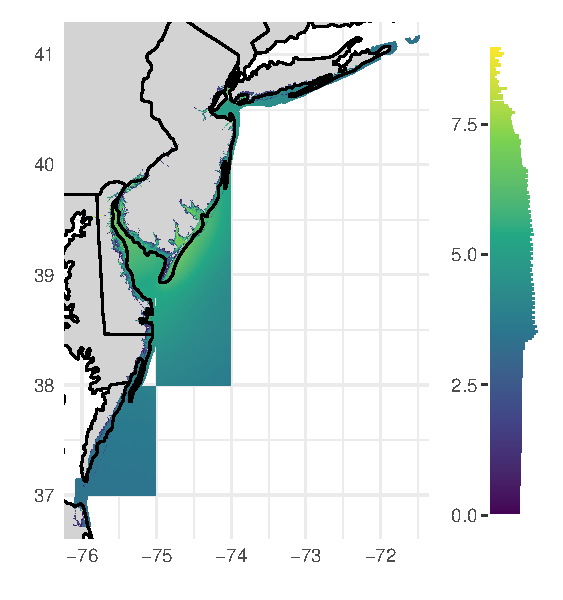
\includegraphics[width=0.99\linewidth]{./plots/slosh1run_loghist}
        \caption{Grid output from one storm simulation in SLOSH, with a marginal
            histogram (with log-scale counts) of surge levels in that storm 
            (truncated at 9 feet).\label{fig:slosh1run}\makenote{add boundaries to indicate
            range of directions and latitudes at which storm makes landfall.}}
    \end{subfigure}%
    ~ 
    \begin{subfigure}[t]{0.48\textwidth}
        \centering
        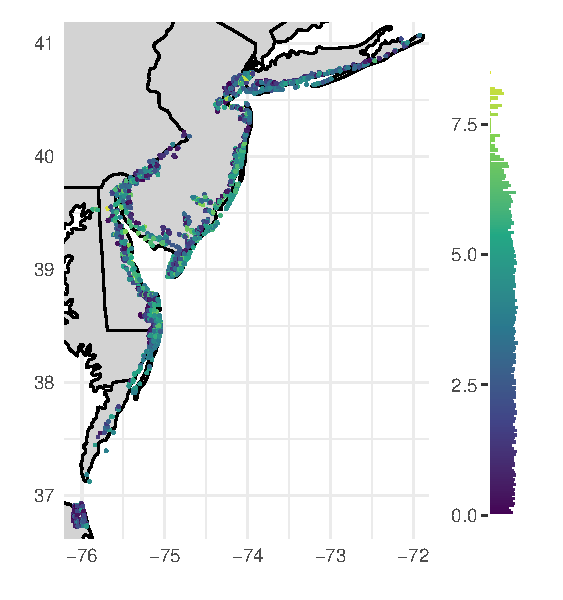
\includegraphics[width=0.99\linewidth]{./plots/sloshthreshold_loghist}
        \caption{
            90th percentile of storm-surge simulations at \num{5283} selected 
            locations with marginal histogram (with log-scale counts).
            \label{fig:sloshthreshold}}
    \end{subfigure}
    \caption{Exploration of SLOSH simulation data.\label{fig:sloshexplore}}
\end{figure}

This paper analyzes SLOSH simulations under an extreme value theory (EVT) framework, 
    using a peaks-over-threshold model.  EVT is a branch of statistics
    that focuses on the tails of the distribution---low density regimes where,
    in this application, the \emph{worst} outcomes occur.  
    We stress here a caveat. EVT assumes that the originating data are independent
    and identically distributed; SLOSH simulations do not meet the second criterion.
    They arise as a result of partially stochastic simulation given a set of input
    parameters---the storm characteristics.  Those storm characteristics themselves
    are sampled via Latin hypercube to fill the allowable parameter space.  That
    having been said, application of the EVT framework to SLOSH still provides us
    with a great deal of information.  It is with that caveat that we continue analysis.
    Figure~\ref{fig:sloshexplore} provides a visual depiction of the SLOSH 
    simulation data.  Figure~\ref{fig:slosh1run} indicates the output of a single 
    storm surge simulation using the SLOSH model. To the right of the map is a 
    histogram (with log-scale counts) displaying observed levels of inundation 
    in the storm, color-coded by the height of the surge at that location.  In this
    plot, there were 45 locations with surge greater than 9 feet above ground level,
    with the maximum value being approximately 19 feet above.  Such occurances
    are highly localized, and are not visible at this scale, so we truncated surge values
    in this plot at 9 feet.  We should also 
    note here that a storm takes some time to occur, and thus values recorded at 
    two locations in a single storm are not necessarily simultaneous.
    In Figure~\ref{fig:sloshthreshold}, we have selected SLOSH grid 
    cells that are in the vicinity of physical features, or locations, of 
    interest.  Displayed are the 90th percentile 
    of inundation for SLOSH simulations at each of those physical features.
    We make clear now, that this analysis is primarily concerned with the
    inferring and applying the dependence structure between storm surge at these locations,
    for storm simulations
    that are in excess of this threshold in at least one identified location.
    Our goal is then a consistent and performant model for multivariate extremes, 
    such that we can learn the dependence structure of extremes in the inundation field.

\makenote{I need to expound upon the necessity/applicability of extreme analysis
    to inundation.  Mention: importance of tails of the distribution, relevance of
    extremes to such analysis, }

The paper proceeds as follows:  Section~\ref{ref:review} details the background 
    for the relevant modelling methods we will be using in this analysis.  In 
    particular, Section~\ref{ref:evt} 
    provides an overview of extreme value theory, to the justification for 
    separating the magnitude of a multivariate extreme from its angular 
    component; Section~\ref{ref:pg} describes the process of creating an angular 
    distribution as well as introducing the model we use in our analysis; and 
    Section~\ref{ref:varbayes} introduces variational Bayesian methods, which we 
    can use to apply our model at large scale. \makenote{rewrite}
    Section~\ref{ref:results} presents our analysis, first demonstrating the 
    efficacy of variational methods on simulated data as compared to MCMC, then
    presenting some interesting results. Finally, Section~\ref{ref:conclusion} 
    concludes.

% EOF 

\section{Review and Background\label{ref:review}}
Our analysis of the SLOSH data's extremal dependence requires some background.  
    \makenote{more appropriate location?}  For 
    convenience, let's also take this opportunity to define some of the notation 
    that will be used throughout the paper.  Let $i = 1,\ldots,n$ iterate over 
    observations in data.  Let $s = 1,\ldots,S$  iterate over dimensions in data.
    In this context, $s$ refers to \emph{sites}, or locations.

\subsection{Extreme Value Theory\label{ref:evt}}
% \begin{comment}
%     \begin{itemize}
%         \item Formal introduction of extreme analysis
%         \begin{itemize}
%             \item Separation of angular and radial components
%         \end{itemize}
%     \end{itemize}
% \end{comment}
\makenote{first paragraph basically copy-pasted from ndpg.  Rephrase more?}
Extreme value theory uses the limited information available in a sample to
    characterize the tails of a distribution.  In the univariate case, asymptotic
    results provide a unique parametric limiting family for the maximum observation
    in a sample.  For data with such a limiting distribution, a common approach
    is to consider observations in excess of a high threshold, and model the
    excesses over that threshold under a generalized Pareto framework.  This
    approach is known as \emph{peaks over threshold} (PoT).  In the multivariate 
    case, the theory for PoT is well established (see, for example, 
    \cite{dehaan2006}), and it indicates the existence of a limiting distribution
    with no parametric representation.  This can pose a challenge for inference,
    but we are not without options.

The multivariate PoT model considered in this paper has been developed 
    in~\cite{trubey:pg}, based on a definition of the limiting distribution proposed
    proposed in~\cite{rootzen2018}.  
    Let $\bm{W} = (W_1,\ldots,W_d)$ be a $d$--dimensional random vector with 
    cumulative distribution $F$.  Assuming there exists a sequence of vectors
    $\bm{a}_n$, $\bm{b}_n$, and a $d$--variate distribution $G$ such that 
    $\lim\limits_{n\to\infty}F^n(\bm{a}_n\bm{w} + \bm{b}_n) = G(\bm{w})$, then
    $G$ is a $d$--variate generalized extreme value distribution.  Then,
    \begin{equation}
        \label{eqn:threshold}
        \lim\limits_{n\to\infty}\text{Pr}
            \left[\bm{a}_n^{-1}(\bm{W} - \bm{b}_n) 
                \leq \bm{w}\mid \bm{W}\not\leq \bm{b}_n\right]
        = \frac{\log G(\bm{w}\wedge \bm{0}) - \log G(\bm{w})}{\log G(\bm{0})}
        = H(\bm{w})
    \end{equation}
    where $H$ is the multivariate Pareto distribution.  \cite{rootzen2018}
    provides a number of stochastic representations of $H$, and in particular,
    Remark~1 justifies the representation given in \cite{ferreira2014} where,
    in the limit, we factorize $\bm{W} = R\bm{V}$ with $R$ and $\bm{V}$ independent.
    \makenote{I'm not very fond of this transition.  We standardize $\bm{W}$ to 
    $\bm{Z}$, then factorize $\bm{Z} = R\bm{V}$.  Separability holds true in both
    cases (i think), but in the former. $\bm{V}$ is still dependent on the marginal 
    distributional parameters.  Standardization allows those to be ignored.  
    We should mention standardization before factorization.}
    $R = \lVert \bm{W}\rVert_{\infty}$ is distributed as a standard Pareto random
    variable, and $\bm{V} = \bm{W} / \lVert \bm{W}\rVert_{\infty}$ is a random
    vector existing within $\mathbb{S}_{\infty}^{d-1}$, the positive orthant of
    the unit sphere under the $\mathcal{L}_{\infty}$ norm.  $R$ and $\bm{V}$
    respectively comprise the \emph{radial} and \emph{angular} components of $H$.
    As $R$ and $\bm{V}$ are independent,  the distribution of $\bm{V}$ is 
    effectively the dependence structure of $\bm{W}$.

Let the threshold $b_{qs} = \hat{F}_{s}^{-1}(1 - q)$, where $\hat{F}$ is
    the empirical cumulative distribution function for the $s$th component.
    Marginally, values exceeding the threshold $b_{qs}$ are assumed to follow
    a univariate generalized Pareto distribution, and are used to estimate the
    corresponding marginal scale and shape parameters $a_{s}$ and $\xi_{s}$
    respectively.  Setting $\bm{b}$ and having inferred $\bm{a}$, and $\bm{\xi}$, 
    we transform $\bm{w}\mid \bm{w}\not\leq \bm{b}$ to a standard multivariate 
    Pareto form via the transformation
    \begin{equation}
        \label{eqn:standardization}
        z_{is} = \left(1 + \xi_{s}\frac{w_{is} 
            - b_{s}}{a_{s}}\right)_{+}^{1 / \xi_{s}}
    \end{equation}
    where $(\cdot)_+$ indicates the positive parts function.  Let 
    $r_i = \lVert \bm{z}_i\rVert$, and $\bm{v}_i = \bm{z}_i / r_i$.  Due to 
    thresholding, $i$ ranges from 1 to $m\leq n$, and $r_i > 1$.  Recall that
    $R\in (1, \infty)$ will, by design, follow a standard Pareto distribution,
    the inferential task left to us is describing the distribution of the
    angular component $\bm{V}\in\mathbb{S}_{\infty}^{d-1}$.  

\subsection{Projected Gamma\label{ref:pg}}
% \begin{comment}
%     \begin{itemize}
%         \item Introduction of Projected gamma distribution
%         \begin{itemize}
%             \item Projected Gamma as the kernel density of a BNP mixture
%         \end{itemize}
%     \end{itemize}
% \end{comment}
A suitable distribution for $\bm{V}$ can be approximated by projecting a 
    distribution in $\mathbb{R}_+^d$ onto $\mathbb{S}_{p}^{d-1}$.  
    Recall the $\mathcal{L}_p$ norm 
    $\lVert \bm{x}\rVert_p = \left(\sum_{s = 1}^dx^p\right)^{1/p}$.  Then
    for $\bm{x}\in\mathbb{R}_+^d$, we define the transformation
    \begin{equation}
        \label{eqn:projection}
        T_p(\bm{x}) = \left(\lVert \bm{x}\rVert_p, 
            \frac{x_1}{\lVert \bm{x}\rVert_p},\ldots, 
                \frac{x_{d-1}}{\lVert \bm{x}\rVert_p}\right)
                =: (r,\bm{y})
    \end{equation}
    where $y = (y_1,\ldots,y_{d-1}) \in \mathbb{S}_{p}^{d-1}$, $r > 0$, and 
    $y_d = (1 - \sum_{s = 1}^{d-1}y_{s}^p)^{\frac{1}{p}}$.
    By transforming $\bm{x}$ to $(r,\bm{y})$ and integrating out $r$, we
    succeed in establishing a distribution for $\bm{y}$ on 
    $\mathbb{S}_{\infty}^{d-1}$
    The Jacobian of the transformation in Equation~\eqref{eqn:projection} is
    $r^{d-1}[Y_d + \sum_{s = 1}^{d-1}y_{s}^py_d^{1-p}]$.
    This Jacobian is well suited to a product of gammas density, where 
    $f(\bm{x}\mid\bm{\alpha},\bm{\beta}) = 
        \prod_{s = 1}^d\mathcal{G}(x_{s}\mid\alpha_{s},\beta_{s})$.
    Transforming $\bm{x}$ as described, $r$ can be integrated out in closed
    form, leaving the \emph{projected gamma} density for arbitrary $p > 0$.
    \[
        f(\bm{y}\mid\bm{\alpha},\bm{\beta}) = \prod_{s = 1}^d\left[
            \frac{\beta_{s}^{\alpha_{s}}}{\Gamma(\alpha_{s})}
            y_{s}^{\alpha_{s} - 1}\right]
            \left[y_d + \sum_{s = 1}^{d-1}y_{s}^py_d^{1-p}\right]
            \frac{\Gamma(\sum_{s = 1}^d \alpha_{s})}{\left(
                \sum_{s = 1}^d\beta_{s}y_{s}
                \right)^{\sum_{s = 1}^d \alpha_{s}}
            }
    \]
    Of course, at $p=\infty$, the transformation is not differentiable, so a 
    direct projection onto $\mathbb{S}_{\infty}^{d-1}$ is not possible. We
    instead desire a high but finite $p$.
    Here we balance two issues: as $p\to\infty$, the space $\mathbb{S}_{p}^{d-1}$ 
    will approach asymptotically towards $\mathbb{S}_{\infty}^{d-1}$.
    Unfortunately, also as $p\to\infty$, the stability of the Jacobian of the
    transformation becomes increasingly dependent on the value, or choice, of 
    $y_d$.  If $y_d\to 0$, then the Jacobian diverges, and the distribution 
    becomes numerically unstable. We select $p = 10$ to balance these concerns.

To more faithfully capture the structure of the data, we use the projected gamma density 
    as a kernel density of an Bayesian non-parametric mixture model, based on 
    the Pitman-Yor process introduced in~\cite{perman1992}.  A Pitman-Yor process
    is a fully atomic measure specified by two parameters and a centering
    distribution.  Under a stick-breaking representation as described 
    in~\cite{ishwaran2001}, 
    \[
        \text{Pr}(\bm{\alpha}\mid\ldots) 
            = \sum_{j = 1}^Jp_j\delta_{\bm{\alpha}_j};\;\;\;
            \sum_{j=1}^Jp_j = 1;\;\;\;
            p_j := \chi_j\prod_{k = 1}^{j-1}(1 - \chi_k)
    \]
    where $\delta_{\bm{\alpha}_j}$ indicates a point mass at $\bm{\alpha}_j$ and
    $\bm{\alpha}_j$ are sampled independently from the centering distribution $G_0$.
    Under the Pitman-Yor process, $\chi_j \sim \text{Beta}(1 - d, \eta + jd)$
    where $d \in [0, 1)$ denotes the \emph{discount} parameter and $\eta > -d$
    denotes the \emph{concentration} parameter.

For the rest of this paper, let $i$ denote indexing over storm simulations (observations), 
    specifically those which survived the thresholding necessitated by the assumption of 
    Equation~\eqref{eqn:threshold}.  Let $s \in \lbrace 1, \ldots, S\rbrace$ denote indexing 
    over locations t which the storm surge is simulated.  That is, $y_{is}$ is the maximum simulated
    storm surge at location $s$ during storm $i$, after projection onto $\mathbb{S}_p^{d-1}$.
    Let $j\in \lbrace 1,\ldots,J\rbrace$ denote indexing over \emph{clusters}, the aforementioned
    mixture components up to truncation point $J$.  Then, the model can be specified as
    \begin{equation}
        \begin{aligned}
            \bm{y}_i \mid \bm{\alpha}_i &\sim
                \mathcal{PG}_p\left(\bm{Y}\mid\bm{\alpha}_i,\bm{1}\right)\\
            \bm{\alpha}_i &\sim G\\
            G &\sim \mathcal{PY}\left(\eta, \zeta, G_0\right)        
        \end{aligned}
        ~\hspace{1cm}
        \begin{aligned}
            G_0 &= {\textstyle\prod}_{s = 1}^{S}\mathcal{G}(\alpha_{s}\mid \xi_{s},\tau_{s})\\
            \xi_{s} &\sim \mathcal{G}(\xi\mid a, b)\\
            \tau_{s} &\sim \mathcal{G}(\tau\mid c, d)
        \end{aligned} 
    \end{equation}
    where $\eta$ and $\zeta$ are respectively the concentration and discount parameters
    of the Pitman--Yor process.  Fitting this model for a moderate number of sites can be 
    accomplished via Markov-chain Monte Carlo methods.  Using the collapsed Gibbs sampler,
    We introduce a latent cluster assignment variable $\delta_i$ for each storm $i$ which 
    indicates which cluster storm $i$ belongs to.  Then the posterior distribution of

\subsection{SLOSH}
\begin{comment}
    \begin{itemize}
        \item More in-depth discussion of dataset
        \begin{itemize}
            \item Break dataset down into 3 levels of analysis; t90, all--but--road--features, airports.
            \item Descriptive statistics thereof
            \item Pitfalls in analysis?
        \end{itemize}
    \end{itemize}
\end{comment}

The projected gamma based model is not an inherently spatial model.  
    \makenote{change reasoning such that we are interested in \emph{specific} locations
    rather than change from grid to specific locations being due to computational
    complexity.}
    As such, rather than holding the entire grid in memory, it makes sense to consider 
    data pertaining only to landmarks of interest.    If one is performing 
    contingency planning in preparation for the storm season, it would be 
    helpful to know the probability of such services being rendered inoperable 
    simultaneously, precisely when they are needed most.  If one is seeking 
    sites for a new service provider, it would be helpful understand the 
    likelihood of a proposed location being rendered inoperable in the same 
    manner.  For these reasons, and considering the computational complexity of 
    a 23 million dimensional model, rather than consider the entire grid of data 
    pertaining to any particular storm, we subset the data to grid cells in the 
    vicinity of such locations of interest.  These locations are gathered from 
    the 2023 US Census Bureau's \emph{TIGER} database \needcite and specifically 
    the point and landmark file.  If a grid cell falls within 70 meters of a location,
    then the grid cell is identified with the location.  If multiple grid cells
    are within 70 meters, then the nearer one is identified with the location.
    Additionally, we select locations, or grid cells, that have experienced at
    at least some inundation in some $q$ proportion of storm simulations.  That is,
    such that $b_{qs} > 0$, for all $s$ of interest.  This restriction arises
    as a consequence of fitting the parameters for the marginal generalized Paretos:
    if the threshold for excesses $b$ is not set above $0$, the likelihood can diverge, 
    and MLE estimation of the parameters suffers. Here we experience another
    tradeoff, the implications of which are explored in 
    Figure~\ref{fig:thresholdselection}.  Setting a higher threshold allows more 
    sites to be included in the analysis, but in turn reduces the number of storm 
    simulations which exceed the threshold in at least one dimension.  This in turn 
    reduces the amount of information available by which we can estimate the 
    dependence structure.  We create several \emph{slices} of the SLOSH data,
    summarized in Table~\ref{tab:datasets}.

\begin{figure}[ht]
    \centering
    \caption{Trade-offs in threshold specification:
    (Left) Proportion of sites with threshold $b_{qs} > 0$ versus $(1 - q)$; 
    (Right) Proportion of storms $\bm{W}_i \not< \bm{b}_q$ versus $(1-q)$.
    \label{fig:thresholdselection}}
    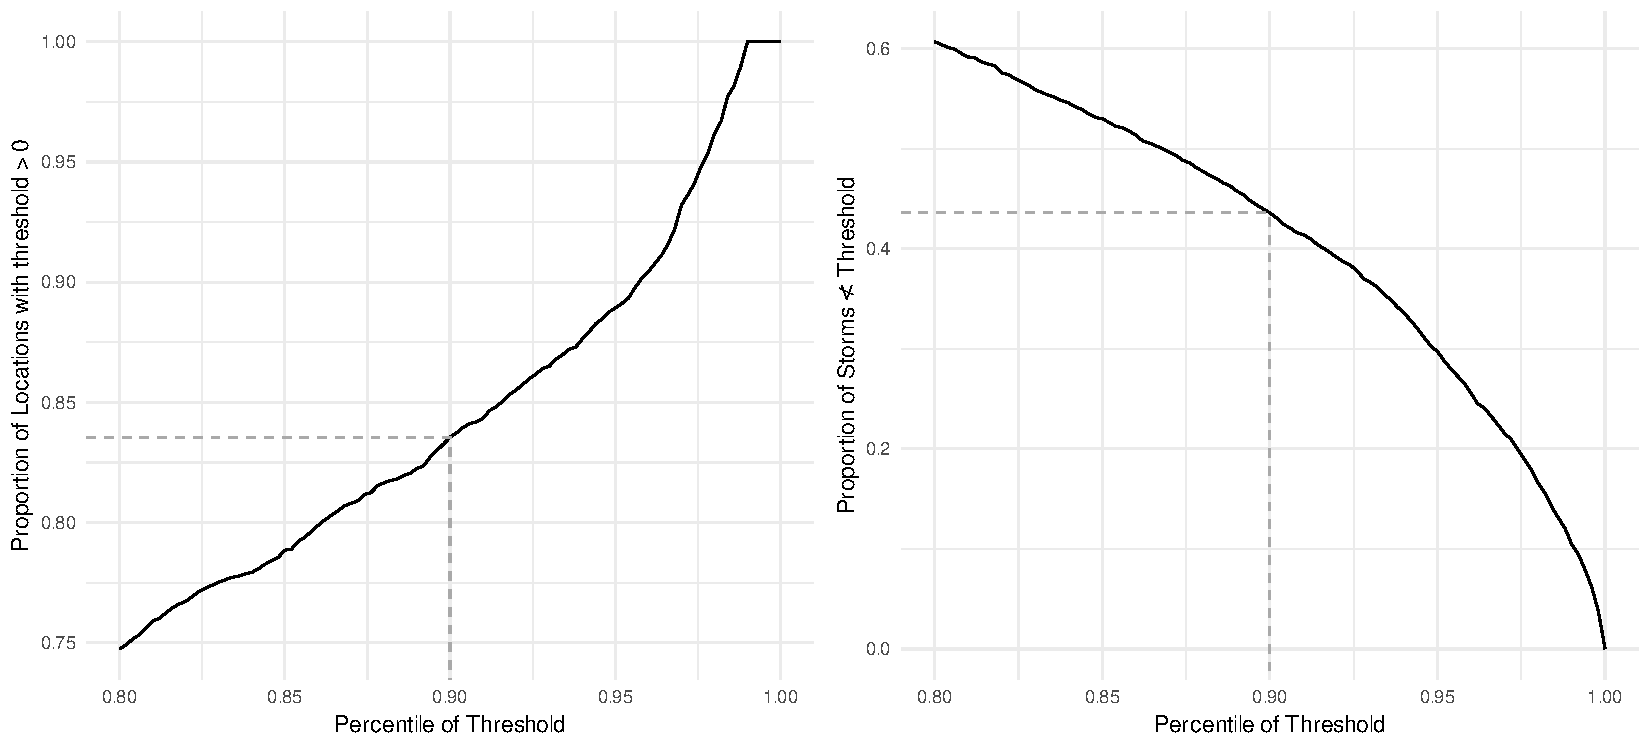
\includegraphics[width=0.9\linewidth]{plots/explore_threshold}
\end{figure}

\begin{table}[htb]
    \centering
    \caption{Slices of SLOSH.  The quantile columns list quantiles \emph{of the threshold}. \makenote{quantiles unnecessary... excise?}\label{tab:datasets}}
    % latex table generated in R 4.4.1 by xtable 1.8-4 package
% Tue Jul 23 14:31:56 2024
\begin{tabular}{lrrrrrrr}
  \hline
Data & Quantile & Cols & Rows & T.05 & T.25 & T.75 & T.95 \\ 
  \hline
Threshold.9 & 0.90 & 4414 & 1744 & 0.39 & 1.64 & 4.58 & 6.19 \\ 
  Limited & 0.95 & 199 & 1040 & 0.38 & 1.84 & 5.13 & 7.00 \\ 
  Transport & 0.95 & 32 & 835 & 0.53 & 1.66 & 5.40 & 6.73 \\ 
  Airports & 0.95 & 27 & 826 & 0.74 & 1.76 & 5.24 & 6.38 \\ 
  Emergency & 0.95 & 6 & 581 & 2.85 & 3.60 & 4.94 & 6.25 \\ 
   \hline
\end{tabular}

\end{table}

At this point, we consider the analysis of the SLOSH data in 3 parts.  First, we
    look at locations pertaining to critical services, or infrastructure, which if 
    rendered unable to operate could drastically increase the negative effects, or 
    loss of life, due to the storm.
    In this context, we are interested in the probability of simultaneous failure.
    For this reason, we look at the transportation and emergency services slices
    of the SLOSH data.
    Second, we look at the overall shape of the inundation field in oder to use
    the clustering action of the Pitman-Yor process to find \emph{emergent} clusters
    of storm characteristics.  That is, we look for groupings of storm characteristics 
    for storms that presented similarly.  For this purpose, we are interested in a large
    sample size, with a large number of locations.  We will be comparing the clustering
    that results from the Threshold.9 and Limited datasets. \makenote{add locality grouping?
    it has better justification than "limited".}
    Realistically, using MCMC methods for model fitting at this scale would be prohibitively 
    expensive, so for that reason we consider a variational approach.
    Finally, \makenote{briefly describe regression goals and why specific datasets.}

\begin{figure}[b]
    \centering 
    \caption{Histograms of characteristics for simulations 
        that survived thresholding in \emph{Threshold.9}.\label{fig:thetahistogram}}
    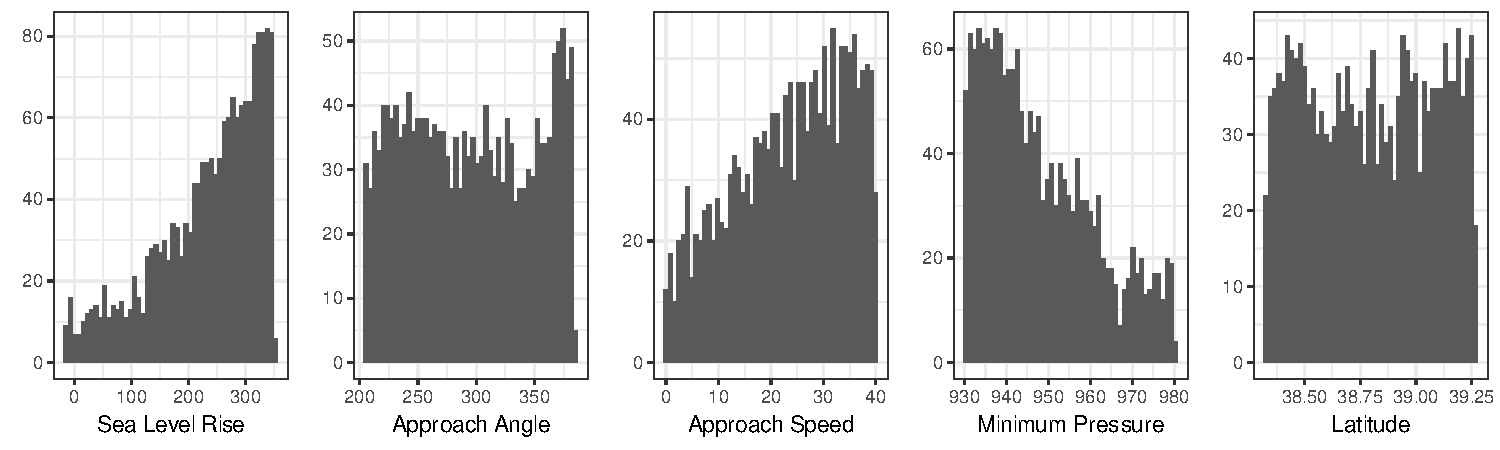
\includegraphics[width=0.9\linewidth]{plots/threshold_histogram}
\end{figure}

Figure~\ref{fig:thetahistogram} shows the marginal histograms of storm parameters, for 
    storms which survived thresholding in the \emph{Threshold.9} slice.  Storm parameters in 
    the originating dataset were sampled via Latin hypercube, so would appear marginally
    uniform.  The difference between marginal uniform, and the observed densities provides
    some indication of what characteristics are necessary for a storm to exceed the threshold.
    In the first case, for sea level rise, it is readily apparent that a higher sea level will
    make it easier for a storm to inundate larger swaths of land, or inundate locations to a
    greater degree.  So we expect to, and in fact do, see a higher probability of a storm exceeding
    the threshold, for a higher sea level rise.  Similarly, a lower minimum pressure in the storm's
    eye corresponds to a more intense storm.  This bears out in a lower minimum pressure having
    a higher percentage of exceeding the threshold.  The relationship to approach speed is 
    interesting in that it's almost linear.  Perhaps, the mechanism there lies in that a higher
    approach speed indicates more power behind the storm.  The spike in approach angle past 360
    degrees is interesting as well. 360 degrees indicates due North, thus approach angles 
    beyond 360 degrees indicate the storm is heading slightly northeast. As these approaches are
    on the eastern seaboard, this means a shallower approach angle relative to the
    land---perhaps offering a given storm more time to inundate larger swaths of land.

% EOF 

\section{Methodology\label{sec:methodology}}
\begin{comment}
    \begin{itemize}
        \item description of joint maxima problem/application
        \item extremal dependence
        \item Multi-site return levels
        \item application results
    \end{itemize}
\end{comment}


        





% EOF

\begin{comment}
    \begin{itemize}
        \item Description of storm parameter clustering problem
        \item Introduction of variational inference
        \begin{itemize}
            \item Describe variational distribution
            \item Necessity (only model using t90 dataset)
            \item Relative performance (computational speed)
        \end{itemize}
        \item Describe clustering methodology
        \item Emergent clusters from both t90 and all--but--road--features in input space.
        \item What does this mean?
    \end{itemize}
\end{comment}

One potential application leveraging use of a Bayesian non-parametric prior is 
    exploiting the clustering inherent to the method. Recall $\delta_i$ is the 
    cluster identifier for observation $i$.  Its sampling is made explicit in
    the MCMC model, though it is integrated out in our variational model. In
    posterior analysis, given $\bm{\alpha}$, and $\bm{\pi}$, where 
    $\pi_j = \nu_j\prod_{k = 1}^{j-1}(1 - \nu_k)$, a probability of cluster 
    assignment can be sampled as
    \begin{equation}
        \label{eqn:clusterprob}
        \text{P}\left(\delta_i = j\mid\bm{\alpha},\bm{\nu},\bm{y}_i\right) 
            = \frac{\pi_j\mathcal{PG}(\bm{y}_i\mid\bm{\alpha}_j,\bm{1})}{
            \sum_{k = 1}^J \pi_j\mathcal{PG}(\bm{y}_i\mid\bm{\alpha}_k,\bm{1})}.
    \end{equation}
    This approach relies on samples of $\bm{\alpha},\bm{\nu}$ from the fitted
    model to generate \emph{loose} clusters for which there is no inherent 
    labelling.  This presents a problem, as interpreting clusters first requires
    \emph{labelling}, or a fixed assignment of observations to clusters.

The variational implementation avoids a label-switching issue inherent to 
    MCMC sampling.  A label-switch between clusters $a$ and $b$ has occured when
    the parameters of clusters $a$ and $b$ have nearly swapped, such that the
    bulk of observations formerly in cluster $a$ are now in cluster $b$, and 
    visa-versa.  This issue does not tend to follow to a variational 
    implementation, as post-fitting, the distributions of cluster parameters are 
    fixed.

With that being the case, a simple option for cluster labelling might be to take
    \[
        \bm{\alpha}_j^* = \frac{1}{S}\sum_{s = 1}^S\bm{\alpha}_{js}\hspace{2cm}
        \bm{\nu}_j^* = \frac{1}{S}\sum_{s = 1}^S \nu_{js},
    \]
    the posterior mean of cluster parameters and cluster weights, then set
    $\delta_i^{*} = \argmax P(\delta_i = j\mid\bm{\alpha}^*,\bm{\nu}^*,\bm{y}_i)$
    as defined in Equation~\eqref{eqn:clusterprob}. We refer to cluster labels
    being assigned in this fashion as \emph{posterior mean clustering}.

Alternative to posterior mean clustering, we could instead take samples of 
    $\bm{\pi}$, $\bm{\alpha}$, then compute 
    $\delta_{is}\mid\bm{\pi}_s,\bm{\alpha}_s$
    as per Equation~\eqref{eqn:clusterprob}.  Then set 
    $\delta_i^{*} = \argmax \mathbbm{1}_{\delta_{is} = j}$.
    We refer to cluster labels being assigned in this fashion as
    \emph{posterior assignment clustering}.  We find, in practice, this method
    results in largely the same label sets as posterior mean clustering.


% EOF

\begin{comment}
    \begin{itemize}
        \item Application of regression analysis? (why?)
        \item introduction of regression model
        \item description of model fitting?  (mcmc description, time?)
        \item results (emergent clusters?)
    \end{itemize}
\end{comment}

\subsection{The Model}
We attempt to develop a flexible regression model on $\mathbb{S}_p^{d-1}$, using the projected gamma as
    the base distribution.  Consider
    \[
        \bm{y}_i \sim \mathcal{PG}(\bm{y}\mid g(\bm{x}_i^T\bm{\theta}), \bm{1})    
    \]
    where $g(\cdot)$ is some linking function that maps $\mathbb{R}\to\mathbb{R}_+$ to maintain the
    viability of inputs for the underlying gamma density.  For our purpose, we use the \emph{softplus}
    function, $g(x) = \log(1 + \exp x)$. The major reason for this choice over the more commonly used
    $\exp(\cdot)$ is numerical: for softplus, small deviations in inputs produce small deviations in
    outputs.  For $\exp(\cdot)$, small deviations in inputs can produce very large deviations in
    outputs.  Some discussion 
    is necessary here as to the dimensionality of $\bm{x}_i$ and $\bm{\theta}$.  Consider a vector 
    $\bm{x}_i$ of dimension $d$, where we might expect each element of $\bm{x}_i$ to contribute to each
    dimension $s$ of $\bm{y}_i$.  We call a model \emph{fully specified} if, for each dimension $s$, we
    have a vector $\bm{\theta}_{is}$, with the same dimensionality as $\bm{x}$.. With some abuse of 
    notation, the fully specified model can be written as
    \[
        \bm{y}_i \sim \int_0^{\infty}
            \prod_{s = 1}^S \mathcal{G}\left(r_iy_{is}\mid g(\bm{x}_i^T\bm{\theta}_{is}), 1\right) \times J(\bm{y}_i) r^{d-1}\text{d}r
    \]
    where $J(\bm{y}_i)$ is the rest of the Jacobian of the projection.  Or more succinctly, 
    \[
        \bm{y}_i \sim \mathcal{PG}\left(\bm{y}_i \mid g((\bm{x}_i \otimes \bm{I}_{S})^T\bm{\theta}), \bm{1}\right)
    \]
    where $\otimes$ denotes the Kronecker product.  To fully realize the flexibility of this model,
    we feature it as the kernel density of a Bayesian non-parametric mixture.
    \begin{equation}
        \label{eqn:regressionmodel}
        \begin{aligned}
            \bm{y}_i &\sim \mathcal{PG}\left(\bm{y}\mid g\left((\bm{x}_i\otimes\bm{I}_S)^T\bm{\theta}_i\right), \bm{1}\right)\\
            \theta_i &\sim G\\
            G &\sim \mathcal{PY}(G\mid\eta, d, G_0)
        \end{aligned}
        ~\hspace{2cm}
        \begin{aligned}
            G_0 &= \mathcal{N}(\bm{\theta} \mid \mu, \Sigma)\\
            \Sigma &\sim \mathcal{IW}(\Sigma\mid \nu, \psi)\\
            \mu\mid\Sigma &\sim \mathcal{N}(\mu\mid \bm{0}, \Sigma / \kappa)
        \end{aligned}
    \end{equation}
    Note the dimensionality of $\bm{\theta}$ under the fully specified model is $d\times S$.
    To explore the efficacy of the regression model, we conduct a minor simulation example using a 
    fully specified model in Figure~\ref{fig:simreg}.  In the left plot, we have the $\bm{x}_i$'s in
    3 distinct clusters. With 2 input dimensions, and 3 output dimensions 
    (with 2 degrees of freedom), $\bm{\theta}$ has a dimensionality of 6. For each cluster
    of inputs, we generate an associated $\bm{\theta}_j$, and project 
    $y_i = g\left((\bm{x}_i\otimes\bm{I}_S)^T\bm{\theta}_j\right) + \bm{\epsilon}_i$ where 
    $\epsilon_{is}$ is a small jitter term onto 
    $\mathbb{S}_{10}^{2}$.  The center plot re-projects that onto $\mathbb{S}_1^{2}$ for display.
    In the right plot, we have the posterior predictive distribution of $\bm{y}_i^{*}\mid \bm{x}_i$.
    We see that we can reasonably recover the original clusters.  In truth, we've given it a hard
    task, as for the fully specified model and the separated nature of the inputs might mean that 
    a single $\bm{\theta}$ vector might reasonably cover 2 or more clusters.  We find 3 emergent
    clusters, with relatively stable cluster assignment that matches the input data.

\begin{figure}[t]
    \centering
    \caption{Posterior predictive distribution under a \emph{fully specified} model, colored 
        by cluster.  Left is the regressors, $\bm{X}$.  Center is 
        $g(\bm{x}_i^T\bm{\theta}_j + \bm{\epsilon}_i)$ projected onto $\mathbb{S}_1^2$.}
    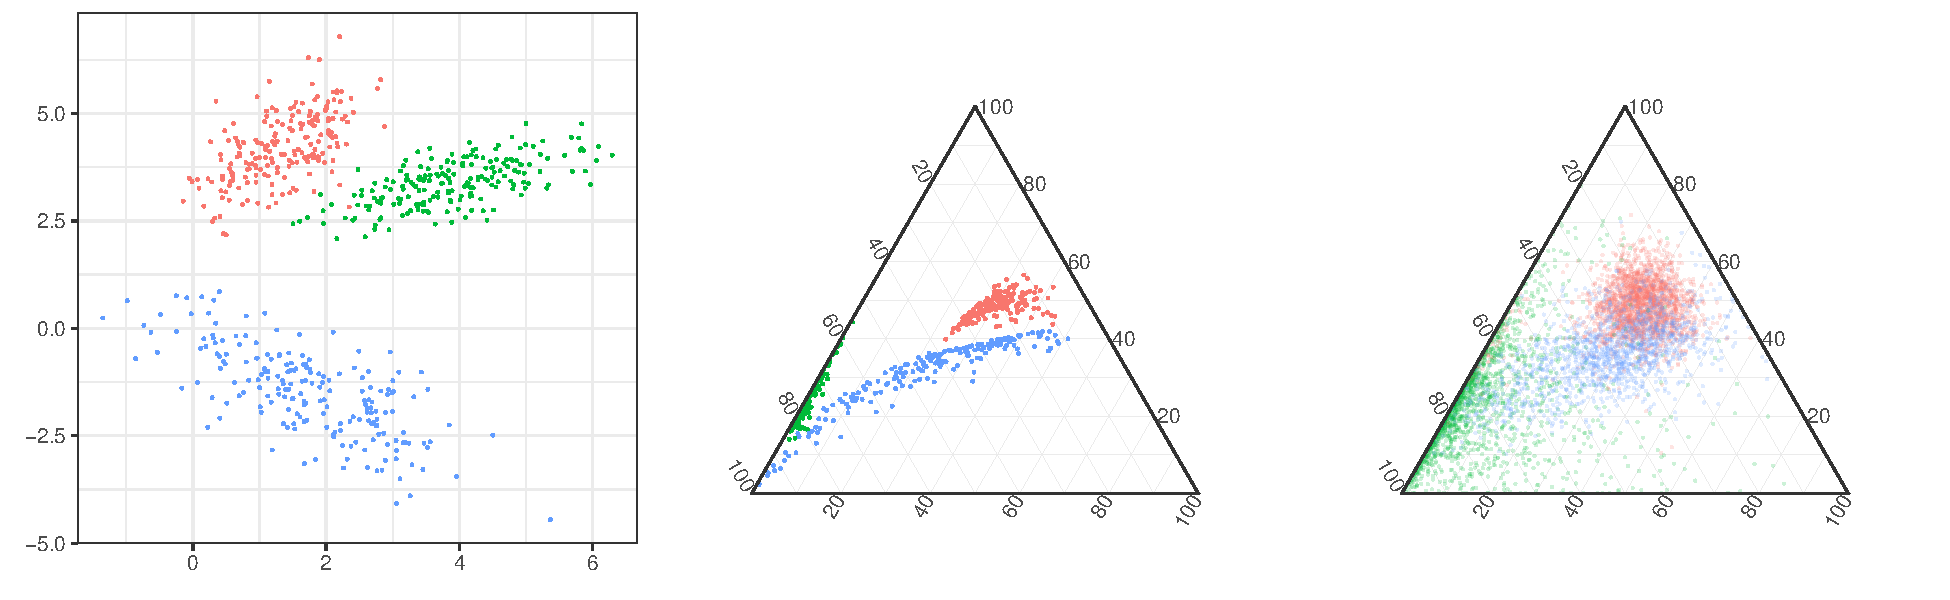
\includegraphics[width = \textwidth]{plots/simulated_reg}
\end{figure}

The fully specified model is extremely inefficient. As $S$ increases, the dimensionality of
    $\bm{\theta}$ increases linearly, which renders it inappropriate for modelling the SLOSH data.  
    However, we can consider other transformations of the data to keep the dimensionality of 
    $\bm{\theta}$ at an appropriate level.
    In the SLOSH data, let $\bm{x}_{is}$, the covariates associated with observation $i$ at location $s$,
    consist of $\bm{x}_{i,\text{obs}}$, the (scaled) parameters under which the $i$th storm is modelled,
    along with $\bm{x}_{s,\text{loc}}$, information pertaining to the $s$th location such as (scaled) 
    latitude and longitude, and $\bm{x}_{is,\text{int}}$, any interaction thereof.  We consider a 
    single linear interaction term between latitude of the storm eye at landfall, and latitude of the
    location $s$.  This results in a $\bm{\theta}$ of dimension $5 + 2 + 1 = 8$.  Then we add
    an additional fixed effect by location, $\varepsilon_s$. Equation~\eqref{eqn:regressionmodelredux}
    summarizes the differences from Equation~\eqref{eqn:regressionmodel} for adapting the regression
    model to SLOSH.
    \begin{equation}
        \label{eqn:regressionmodelredux}
        \bm{y}_i \sim 
            \mathcal{PG}\left(\bm{y}\mid g(\bm{x}_i^T\bm{\theta}_i + \bm{\varepsilon}), \bm{1}\right)
            \;\hspace{1cm}\;
            \varepsilon_s \sim \mathcal{N}(\varepsilon \mid 0, \sigma_{\varepsilon}^2)
    \end{equation}
    where $\bm{x}_i$ is overloaded as discussed.  


    


\section{Results\label{ref:results}}
\subsection{Simulation Study}
To validate the variational model, we conduct a simulation study.
    As we are interested in an angular model, the data is generated from 
    a finite mixture of projected gammas distribution, at varying levels
    of dimensionality and number of mixture components.  For each simulation,
    1000 replicates are sampled. In Figure~\ref{fig:energyscore} we compare the 
    rise in energy score of the fitted model over a baseline energy score,
    computed as the energy score between two datasets generated from the same
    distribution.  The higher the quality of recovery of the generating
    distribution, the closer the \emph{rise} in energy score would be to zero.
    For each number of mixture components and number of columns, there are 10 
    such simulations.  The rise over baseline energy score reported is averaged
    over those 10 simulations.

\begin{figure}[ht]
    \caption{Rise in energy score over baseline (Y) versus dimensionality (X), 
            by number of latent mixture components in generating distribution
            \label{fig:energyscore}}
    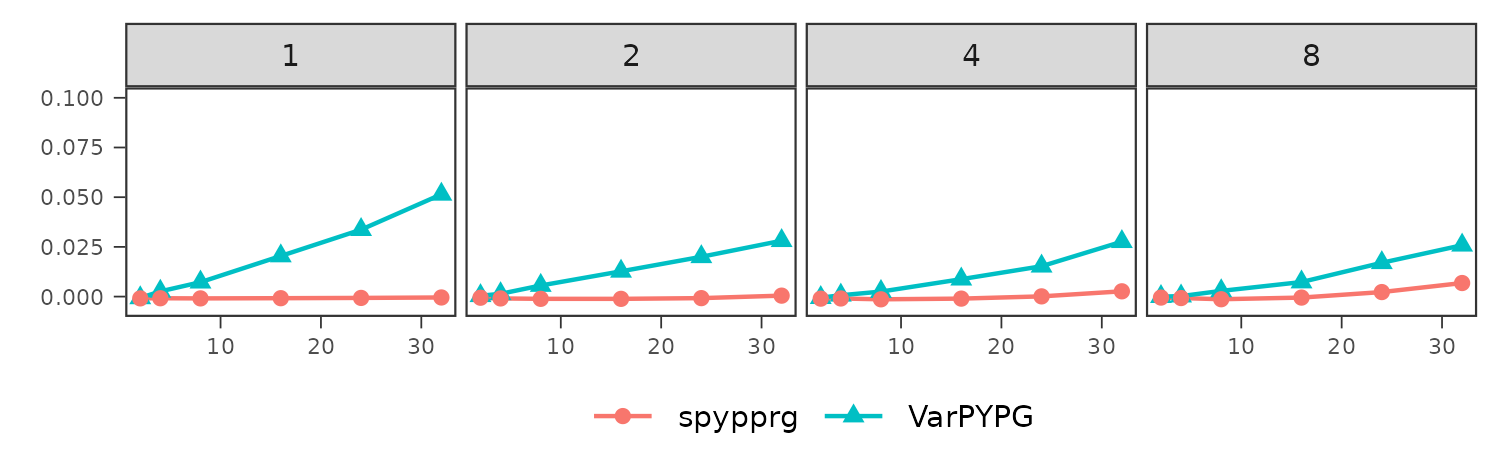
\includegraphics{./plots/energy_score}
\end{figure}

\makenote{need to put in a comparative model to make the variational model not
    look as bad by comparison.}
We see the MCMC model nearly perfectly captures the original distribution as
    measured by energy score.  The variational model is not far behind, however.

% EOF

\section{Conclusion\label{ref:conclusion}}
\begin{comment}
    \begin{itemize}
        \item Desire for more comprehensive data (additional sources of flooding?  rain?)
        \item Value in each model approach
        \item Additional steps to be taken / model extensions worth exploring
    \end{itemize}
\end{comment}

% EOF

\appendix
% \section{Accompanying math in support of the mixed variational method}
% \begin{equation}
%     \begin{aligned}
%         f(\bm{y},\theta\mid\phi) &\propto \mathcal \prod_{j = 1}^J\left[\prod_{i:\gamma_i = j}\left[\mathcal{PG}(\bm{y}_i\mid\bm{\alpha}_j,\bm{1})\right]\times\prod_{\ell = 1}^d\mathcal{G}(\alpha_{j\ell}\mid\xi_{\ell},\tau_{\ell})\right] \\
%         &\hspace{1cm}\times \left[\prod_{\ell = 1}^d\mathcal{G}(\xi_{\ell}\mid a, b)\mathcal{G}(\tau_{\ell}\mid c,d)\right]        
%     \end{aligned}
% \end{equation}
% After expansion, $\log f(\bm{y},\theta\mid\phi)$ becomes
% \begin{equation}
%     \begin{aligned}
%     \log f(\bm{y},\theta\mid\phi) &= \sum_{j = 1}^J\Biggl[
%     \sum_{i:\gamma_i = j}\left[\log\Gamma(\bm{1}^T\bm{\alpha}_j) - (\bm{1}^T\bm{\alpha}_j)\log(\bm{1}^T\bm{y}_i)\right]\\
%     &\hspace{2cm}+ \sum_{\ell = 1}^d\left[(\alpha_{j\ell} - 1){\small\sum}_{i:\gamma_i = j}\log(y_{i\ell}) + n_j\log\Gamma(\alpha_{j\ell})\right]\\
%     &\hspace{2cm}+ \sum_{\ell = 1}^d\left[\xi_{\ell}\log(\tau_{\ell}) - \log\Gamma(\xi_{\ell}) + (\xi_{\ell} - 1)\log(\alpha_{j\ell}) - \tau_{\ell}\alpha_{j\ell})\right]
%     \Biggr]\\
%     &\hspace{1cm}+ \sum_{\ell = 1}^d\left[a\log(b) - \log\Gamma(a) + (a - 1)\log(\xi_{\ell}) - b\xi_{\ell}\right]\\
%     &\hspace{1cm}+ \sum_{\ell = 1}^d\left[c\log(d) - \log\Gamma(c) + (c - 1)\log(\tau_{\ell}) - d\tau_{\ell}\right]   
%     \end{aligned}
% \end{equation}
% Then the gradient may be evaluated as follows:
% \begin{equation}
%     \begin{aligned}
%         \frac{\partial}{\partial \alpha_{j\ell}} \log f(\bm{y},\theta\mid\phi) &= \sum_{i:\gamma_i = j}\left[\psi(\bm{1}^T\bm{\alpha}_j) - \log(\bm{1}^T\bm{y}_i)\right]\\
%         &\hspace{1cm}+ \sum_{i:\gamma_i = j}\log(y_{i\ell}) + (n_j + \xi_{\ell} - 1)\psi(\alpha_{j\ell})\\
%         \frac{\partial}{\partial \xi_{\ell}}\log f(\bm{y},\theta\mid\phi) &= J\left(\log(\tau_{\ell}) - \psi(\xi_{\ell})\right) + \sum_{j = 1}^J\log(\alpha_{j\ell}) + \frac{a - 1}{\xi_{\ell}} - b\\
%         \frac{\partial}{\partial \tau_{\ell}}\log f(\bm{y},\theta\mid\phi) &= \frac{J\xi_{\ell} + c - 1}{\tau_{\ell}} - \sum_{j = 1}^J \alpha_{j\ell} - d        
%     \end{aligned}   
% \end{equation}
% where $\psi(\cdot)$ is the the digamma function.

% Letting $q(\log \alpha_{j\ell}) = \mathcal{N}(\mu_{\alpha_{j\ell}},\sigma_{\alpha_{j\ell}})$, 
%     or rather $\alpha_{j\ell} = \exp(\mu_{\alpha_{j\ell}} + \sigma_{\alpha_{j\ell}}\varepsilon$ 
%     where $\varepsilon \sim \mathcal{N}(0,1)$, we can create a mean-field approach for the
%     cluster shape parameters, and prior shape and rate parameters, while maintaining exact
%     sampling of the cluster membership parameters.

% EOF 

\bibliographystyle{chicago}
\bibliography{./refs}

\end{document}

% EOF